%   File: Golfer.tex
% Author: Adam Leeper
%------------------------------------------------------------------------------
%\\[0.45pc]
\providecommand{\isolatedBuild}[1]{#1}% Fallback definition to build normally.
\isolatedBuild{
  \documentclass[11pt,letterpaper]{book}
  %\documentclass[11pt,letterpaper]{book}

% aleeper: I think these are needed for Paul's macros?
\usepackage{epsfig}
\usepackage{epstopdf}

%\makeatletter
%\typeout{The import path is \import@path}
%\makeatother

\usepackage{import}

\subimport{./}{packagesMitiguy.sty}
\subimport{./}{macrosMitiguy.tex}
\subimport{./}{PageStylesMitiguy.tex}
\subimport{./}{macrosLeeper.tex}
   % Found via TEXINPUTS environment variable.
  \isolatedBuildHeader{Velocity Constraints and Rolling}
                      {Amusement Park: Ship Ride}
}
%%%
%%%
%%%
{
\small
\begin{minipage}[t]{0.6\linewidth}
  \minipageTopAnchor
  A common theme-park ride is pictured below.
  The ride features a ship, \basis{B}, that swings from a top support, $B_o$,
  fixed in a Newtonian reference frame \basis{N}, as pictured.
  A tire \basis{A}, whose center $A_o$ is fixed in \basis{N}, makes contact
  with the bottom of the ship.
  Hence, the angular motion of the tire is used to swing the ship back and
  forth.
  %
  \\[0.5pc]
  During a certain interval, the \textbf{counter-clockwise} rotation rate of
  the tire is described by $\omega_A = 10*\sin(t)$.
  The radius of the tire is $R_A = 0.3$ m.
  %
  \\[0.5pc]
  Let the \textbf{counter-clockwise} rotation rate of the ship be denoted by
  $\omega_B$. The distance from $B_o$ to the bottom surface of the ship is
  $R_B = 6$ m.
  %
  \\[0.5pc]
  Right-handed orthogonal unit vectors \uvecxyz{n} are fixed in \basis{N}
  as shown.
  %
%  \begin{center}
%    \includegraphics[height=6cm]{mayflower.jpg}
%    \hspace{1cm}
%    \includegraphics[height=6cm]{boat.png}
%  \end{center}
  %
  %\\[0.5pc]
  \begin{itemize}
    \item \textbf{Calculate} the velocity of the point of the tire in contact
      with the ship, $\vel{A_B}{N}$.
      %
    \item \textbf{Calculate} the velocity of the point of the ship in contact
      with the tire, $\vel{B_A}{N}$.
      %
    \item When the ship \textbf{rolls} on the tire, write the relevant
      \textbf{constraint equation} and use it to find a \textbf{scalar}
      relationship between $\omega_A$ and $\omega_B$.
      %
    \item \textbf{Compute} $\omega_B$ and $\alpha_B$ when $t = \frac{\pi}{6}$
      seconds.
  \end{itemize}
\end{minipage}
\hfill
\begin{minipage}[t]{0.35\linewidth}
  \minipageTopAnchor
  \includegraphics[width=1.0\linewidth]{mayflower.jpg}
  \\[1.5pc]
  \includegraphics[width=1.0\linewidth]{boat.png}
\end{minipage}
}
%
\isolatedBuildFooter